\newpage
\subsection{(R) Avoidance Grid Run}\label{s:aviudabceGridRun}
\paragraph{Main Goal:} The main goal of this section is to introduce the trajectory selection process, based on a \emph{situation assessment}, originating from \emph{Data Fusion Procedure} (sec. \ref{s:sensorFusion}). 

\begin{note}
    The \emph{rating calculation} is outlined in (sec. \ref{s:sensorFusion}). Low cost sensor fusion example usable to feed our data fusion procedure is given in \cite{sabatini2013low}. Semi-optimal concatenation trajectory search  like ours can be found in \cite{shaw1998using}.
\end{note}

\begin{figure}[H]
\centering
    \begin{subfigure}{0.48\textwidth}
        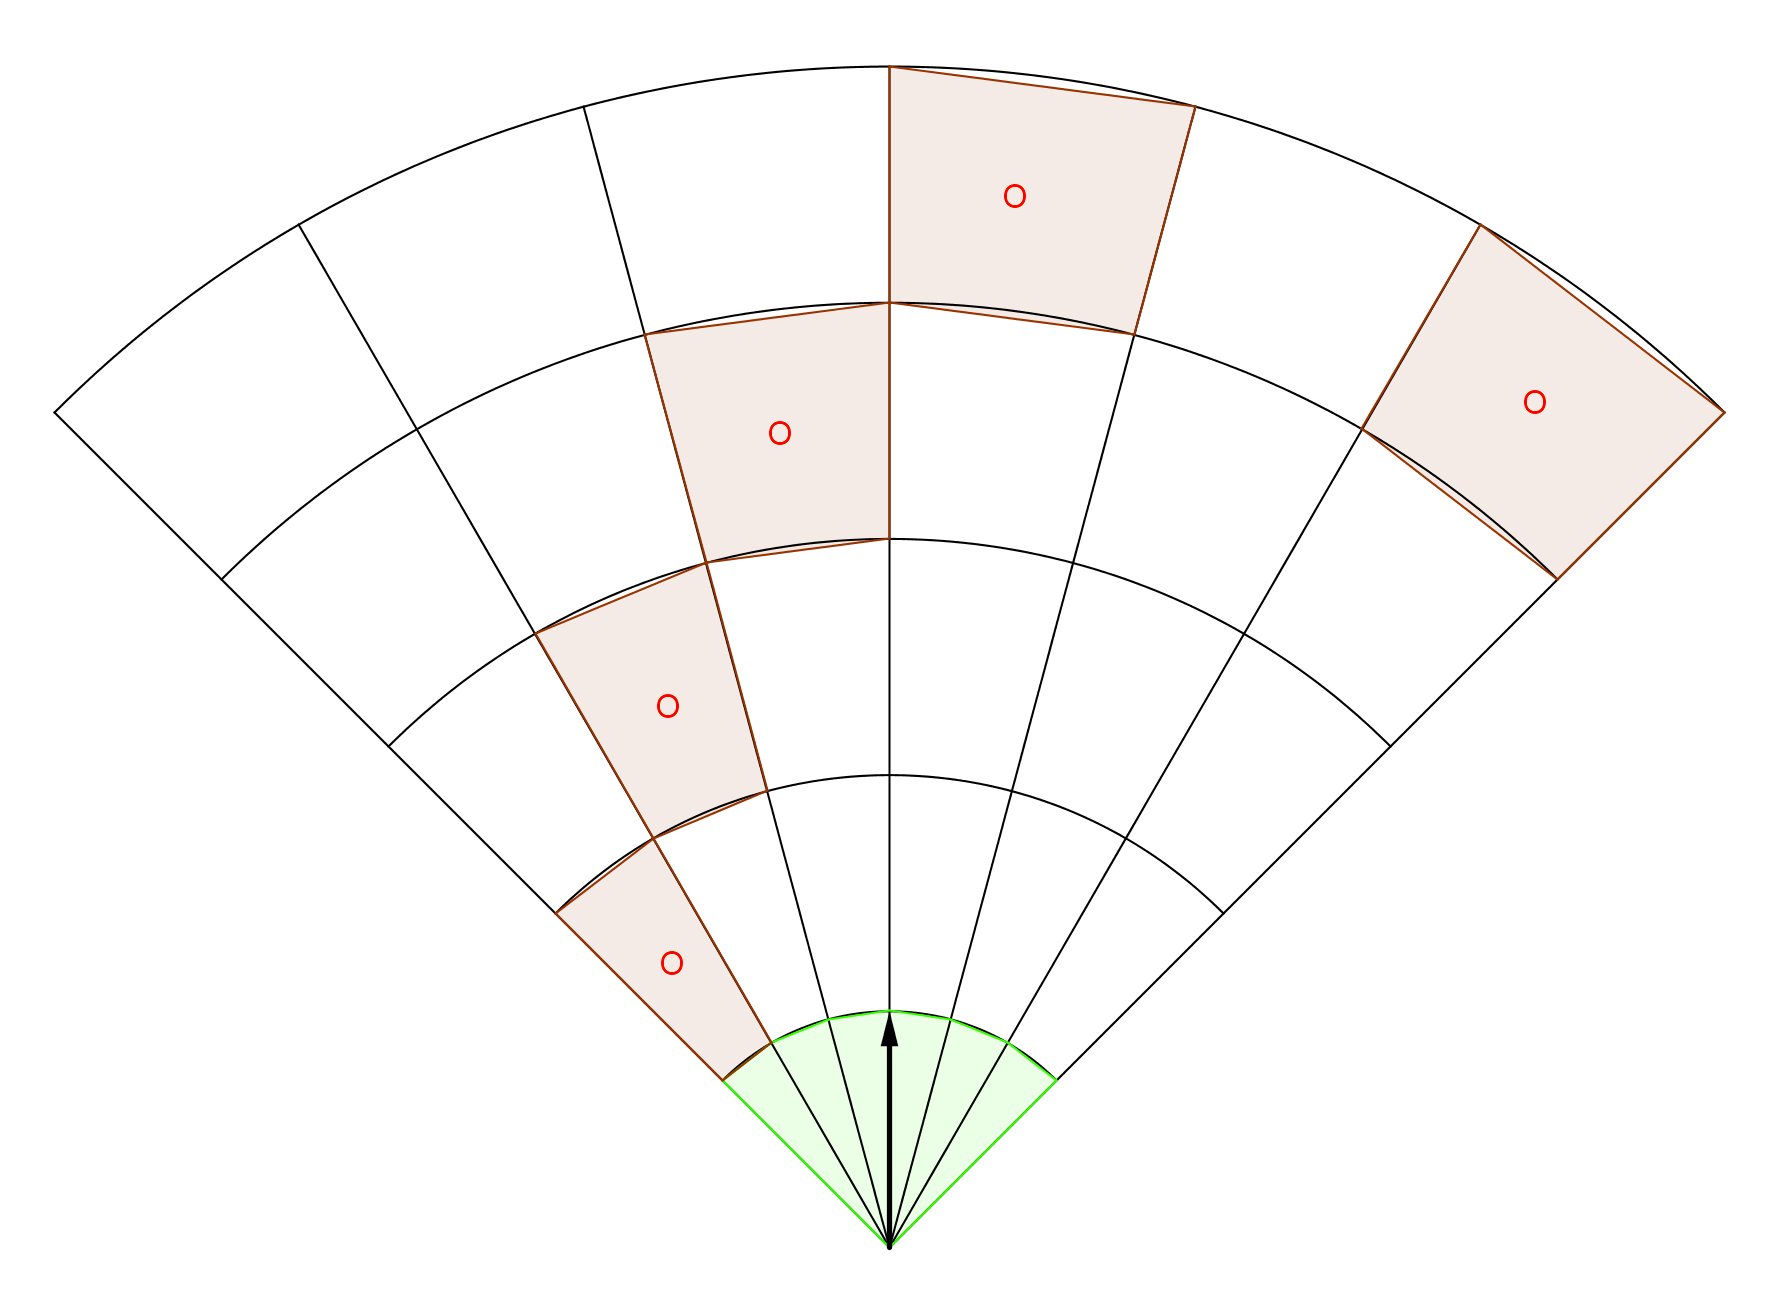
\includegraphics[width=0.9\linewidth]{\FIGDIR/CA001ObstacleDetection}
        \caption{Obstacle detection.}
        \label{fig:obstacleDetectionAvoidanceGrid}
    \end{subfigure}
    \begin{subfigure}{0.48\textwidth}
        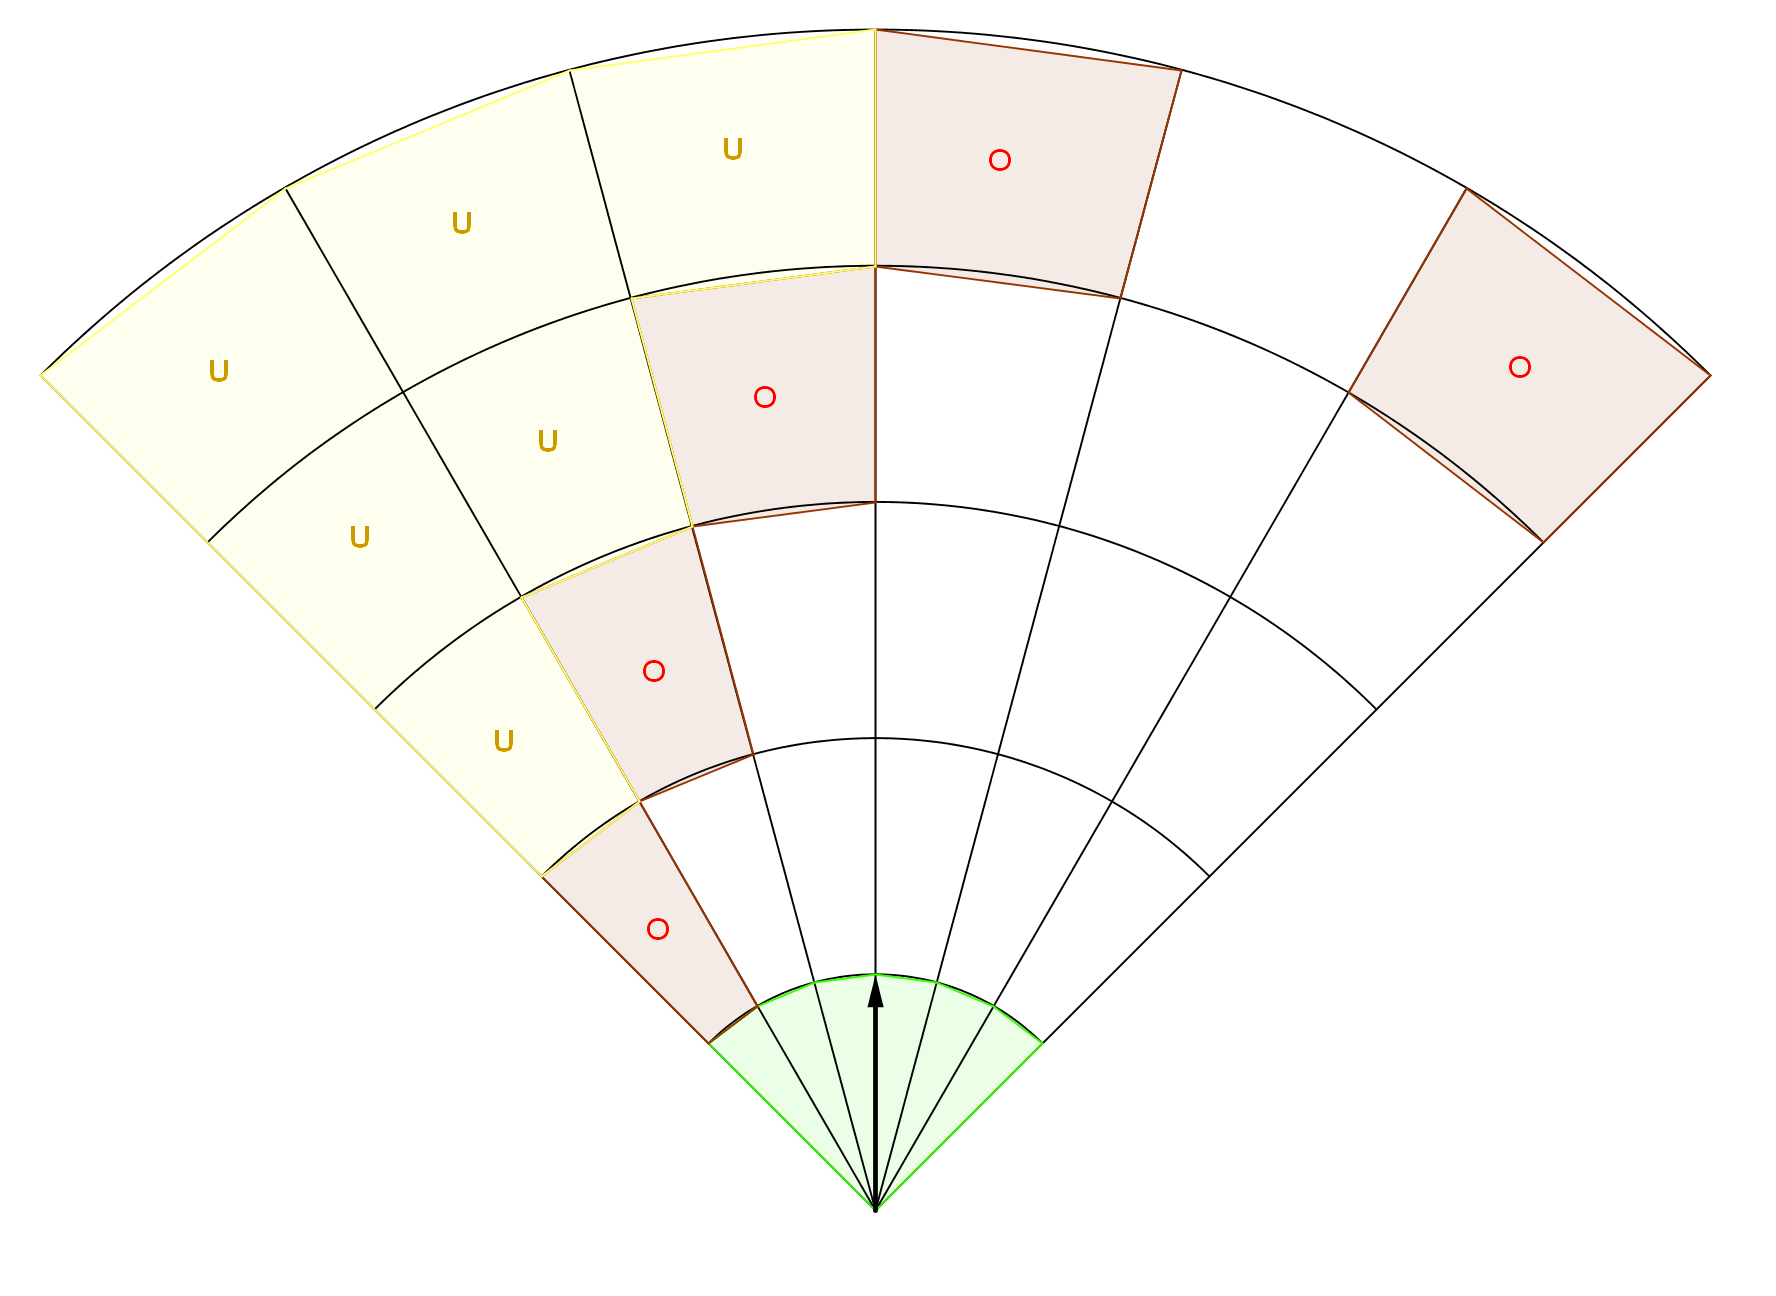
\includegraphics[width=0.9\linewidth]{\FIGDIR/CA002UncertainityAssesment} 
        \caption{Uncertainty assessment.}
        \label{fig:uncertainityAssesmentAvoidanceGrid}
    \end{subfigure}
    \\
    \begin{subfigure}{0.48\textwidth}
        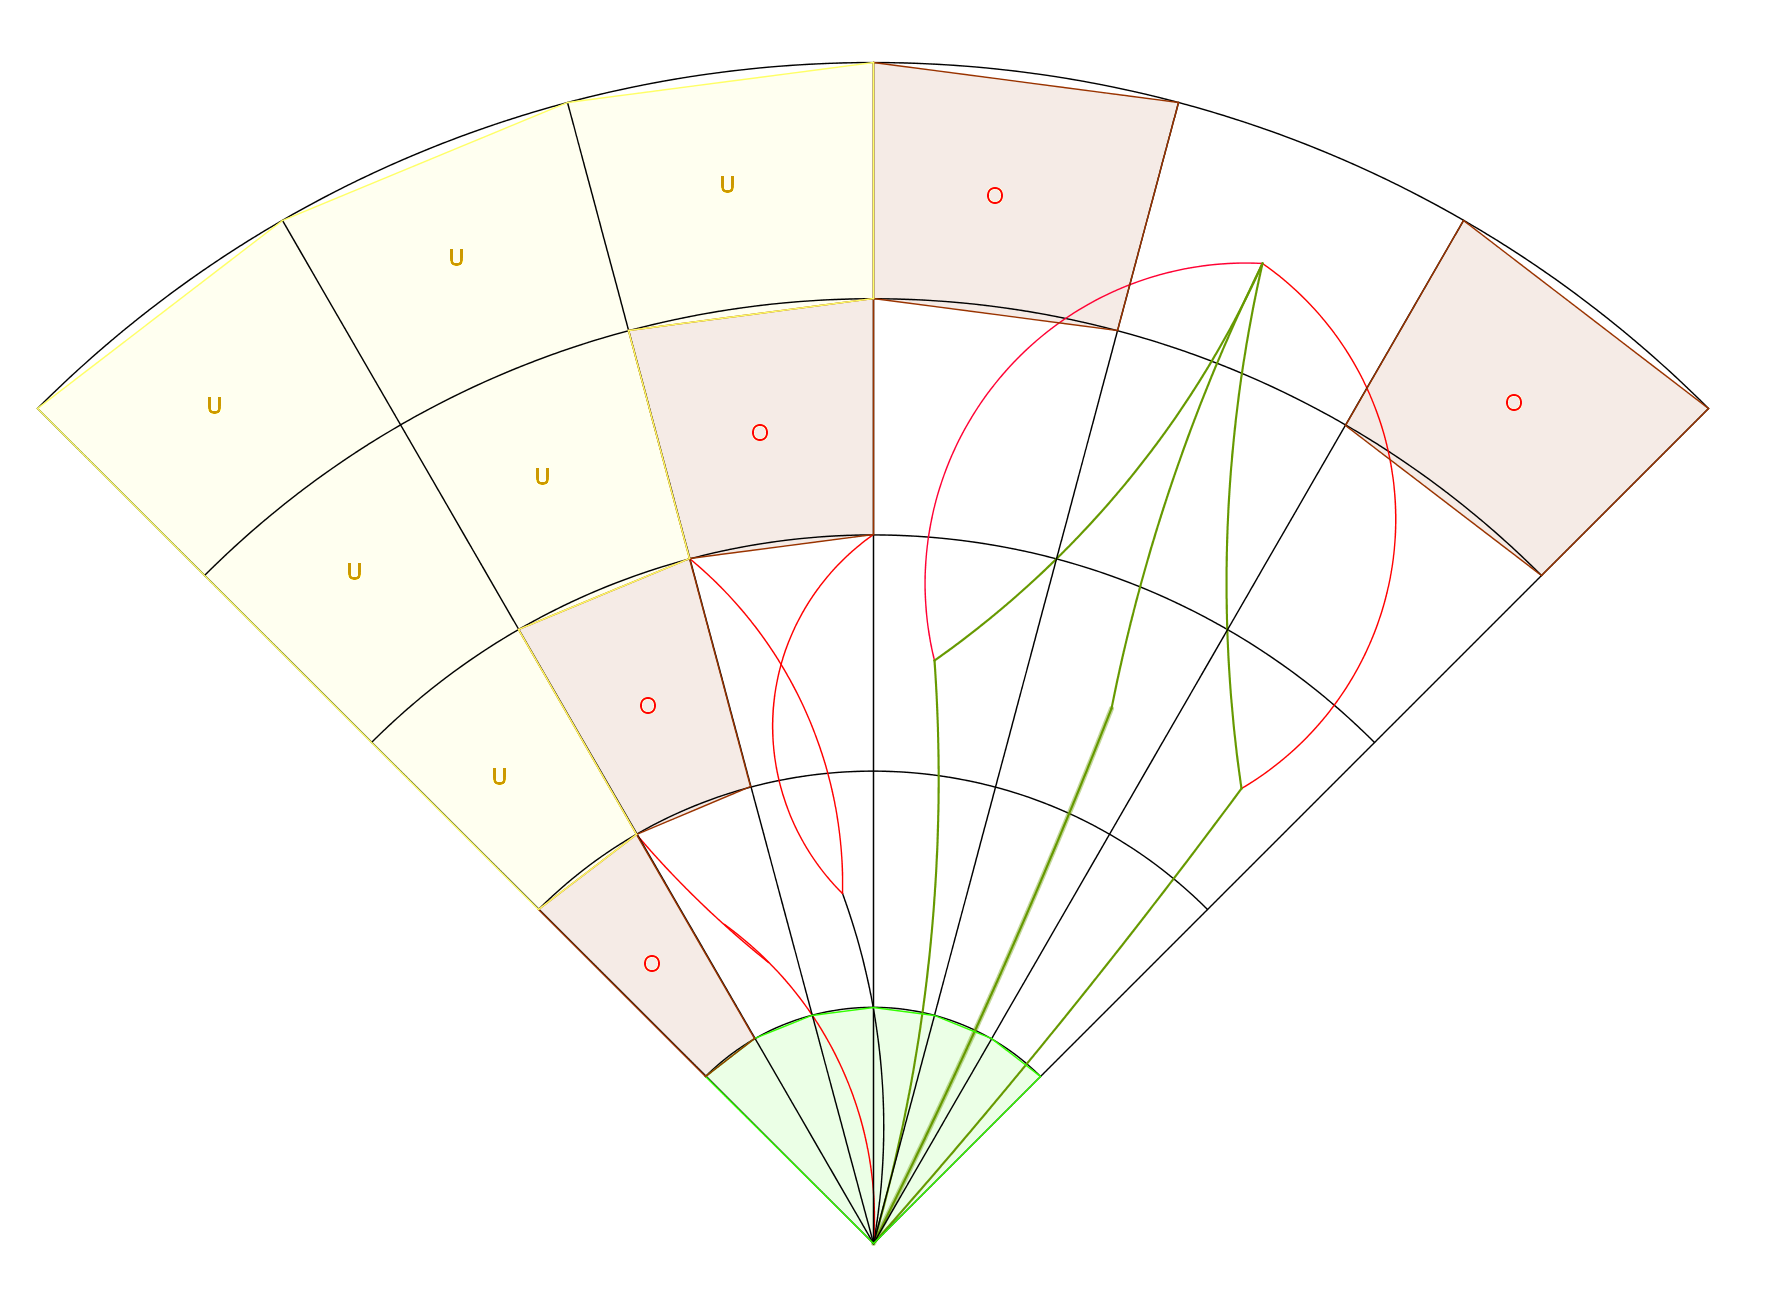
\includegraphics[width=0.9\linewidth]{\FIGDIR/CA003SurveyOfVacantSpace} 
        \caption{Trajectories reachibility evaluation.}
        \label{fig:trajectoriesSafetyEvaluationAvoidanceGrid}
    \end{subfigure}
    \begin{subfigure}{0.48\textwidth}
        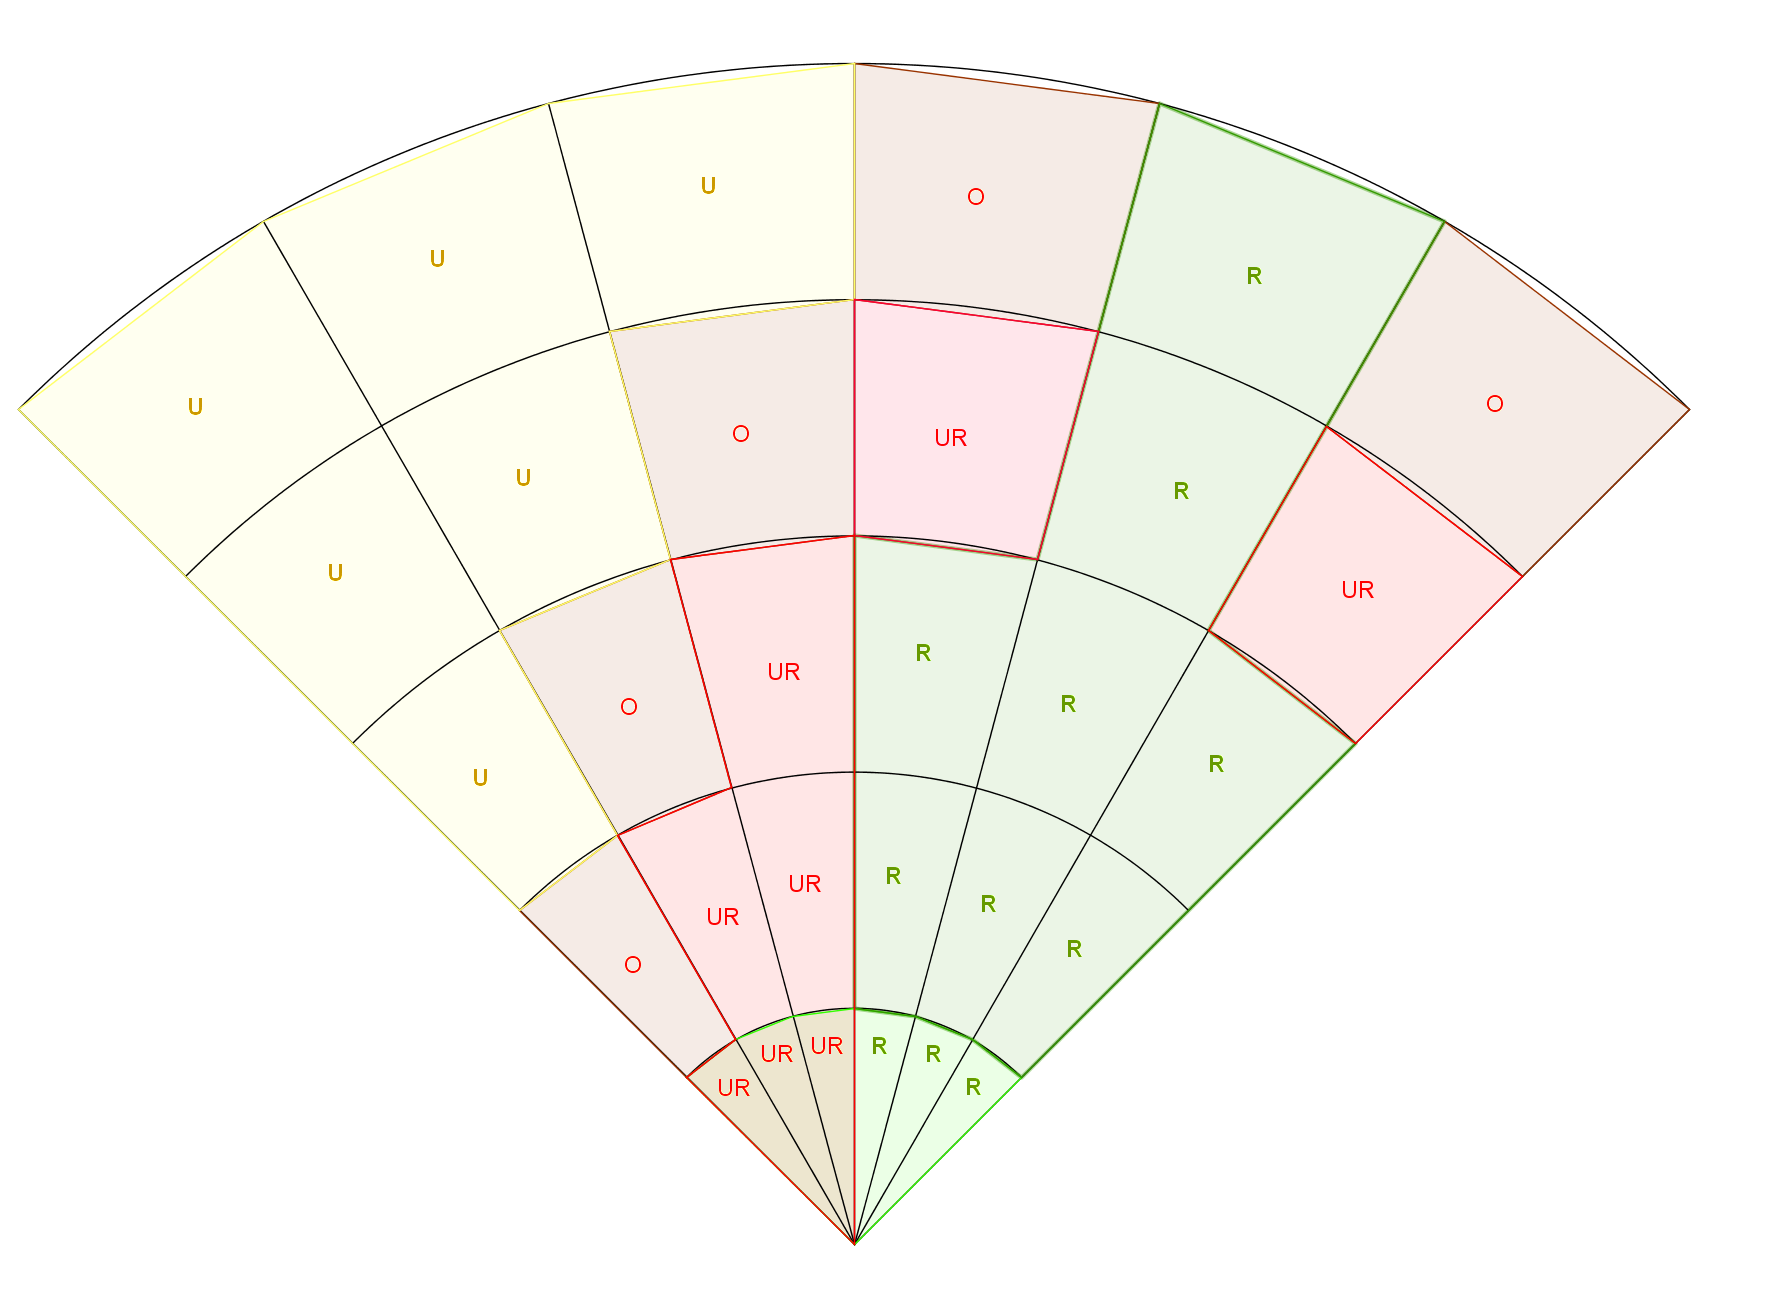
\includegraphics[width=0.9\linewidth]{\FIGDIR/CA004ReachableSpaceAssesment} 
        \caption{Cell reachibility evaluation.}
        \label{fig:reachibilityAssessmentAvoidanceGrid}
    \end{subfigure}
    \caption{Significant steps of \emph{Avoidance grid run} (inner loop).}
    \label{fig:significantStepsofAvoidanceGridRun}
\end{figure}

\begin{note}
    The \emph{Sensor Fusion Procedure} is solving all following steps (sec. \ref{s:sensorFusion}). The \emph{main purpose} of \emph{Avoidance Run} is finding best path under certain conditions.
\end{note}

\paragraph{Space Assessment Principle:} The \emph{Avoidance Grid} is fed trough \emph{Data Fusion} (sec. \ref{s:sensorFusion}). The process of \emph{ratings assessment} (tab. \ref{tab:defuzificationRatings}) is given in (fig. \ref{fig:significantStepsofAvoidanceGridRun}):
\begin{enumerate}
    \item \emph{Obstacle detection} (fig. \ref{fig:obstacleDetectionAvoidanceGrid}) - assessment of \emph{detected obstacles} (eq. \ref{eq:detectedObstacleRatingForCell}). The red (O) $cells$ have Detected obstacle set as \emph{true}. The other threats: \emph{map obstacles} (eq. \ref{eq:mapObstacleRatingForCell}), \emph{intruders} (eq. \ref{eq:intruderRatingForCell}), \emph{constraints} (eq. \ref{eq:constraintRatingForCell}) are false. The red (0) $cells$ are representing $Occupied(t_i)$ (eq. \ref{eq:ocuupiedDataFusion}) space in \emph{Avoidance Grid} at decision time $t_i$.
    
    \item \emph{Uncertainty assessment} (fig. \ref{fig:uncertainityAssesmentAvoidanceGrid}) - the uncertain cells are cells which status can not be \emph{assessed}. The \emph{Visibility} (eq. \ref{eq:visibilityForCell}) is low. The \emph{Uncertain} cells (yellow (U) mark) are equal to $Uncertain(t_i)$ (eq. \ref{eq:UncertainDataFusion}) in \emph{Avoidance Grid} in \emph{decision time} $t_i$. The $Constrained(t_i)$ (eq. \ref{eq:ocuupiedDataFusion}) space is equal to $\varnothing$ in this example.
    
    \item \emph{Trajectory reachibility evaluation} (fig. \ref{fig:trajectoriesSafetyEvaluationAvoidanceGrid}) - the \emph{Reach Set} given as \emph{Trajectory Set} (eq. \ref{eq:trajectoryTree}). is then projected trough \emph{Avoidance Grid} and pruned according to (def. \ref{def:PrunedReachSet}). \emph{Reachable Trajectories} (eq. \ref{eq:trajectoryReachibility}) are only those contained in $Free(t_i)$ space (eq. \ref{eq:freeDataFusion}). The \emph{Reachable Trajectories} are denoted as \emph{green lines}. The \emph{Unreachable} trajectory segments are denoted as \emph{red lines}. 
    
    \item \emph{Cell reachibility evaluation} (fig. \ref{fig:reachibilityAssessmentAvoidanceGrid}) - the evaluation of $cells$ reachibility is going according to (eq. \ref{eq:cellReachibility}). The \emph{Reachable cells} are those which \emph{contains} at least one \emph{Reachable Trajectory Segment}.
\end{enumerate}



\paragraph{Finding Best Path:} \footnote{Avoidance Run Function Implementation:\url{RuleEngine/MissionControl/MissionControl.m::findBestPath(avoidanceGrid)}} Each $cell_{i,j,k}$ in \emph{Avoidance Grid} at \emph{decision time} $t_i$ has assessed ratings according to \emph{data fusion procedure} (tab. \ref{tab:defuzificationRatings}). The following properties are know prior the \emph{trajectory} selection:
\begin{enumerate}
    \item \emph{Reachibility} for each  $cell_{i,j,k}$ (eq. \ref{eq:cellReachibility}).
    \item \emph{Reachibility} for each  $Trajectory(\circ)$ (eq. \ref{eq:trajectoryReachibility}).
    \item \emph{Free Space} as non empty set of $cells$ in \emph{Avoidance Grid} (eq. \ref{eq:freeDataFusion}), with \emph{Reachable Space} (eq. \ref{eq:ReachableDataFusion}).
    \item \emph{Goal Waypoint} $\mathscr{WP}_G$ from \emph{Mission Control Run} (sec. \ref{s:missionControlRun}).
\end{enumerate}

The \emph{Algorithm} (alg. \ref{alg:FindBestPathAvoidanceGrid}) is based on \emph{shortest path} search. Navigation is trying to reach \emph{goal waypoint}, therefore it tries to shorter distance between \emph{trajectory final cell} and \emph{goal waypoint}. If there is \emph{reachable space} two situations can occur:
\begin{enumerate}
    \item \emph{Goal waypoint is inside the Avoidance Grid} - the \emph{avoidance cell} is cell$_{i,j,k}$ containing \emph{goal waypoint} if reachable. 
    
    \item \emph{Goal waypoint is outside the Avoidance Grid} - the \emph{avoidance cell} is closest cell considered as \emph{outer cell} to \emph{goal waypoint}.
\end{enumerate}

\begin{note}
    \emph{Outer cell} is a cell$_{i,j,k}$ which has at least one \emph{wall} directly neighbouring with \emph{outer space} ($Universe - Known World (t_i)$). The \emph{outer cell} is selected to prevent navigation to the \emph{trap}.
\end{note}

The \emph{Avoidance Path} selection is simple lowest cost selection of \emph{Trajectory} $\in$ cell$_{i,j,k}$.
\newpage

\begin{algorithm}[H]
\SetKwInOut{Input}{Input}
\SetKwInOut{Output}{Output}
\Input{Cell[]  reachable (eq. \ref{eq:ReachableDataFusion}), Waypoint goal, AvoidanceGrid($t_i$) grid}
    
\Output{Trajectory avoidancePath, Error message}
    
    \BlankLine
    \# Initialization \& Reachibility test\;    
    avoidancePath = $\varnothing$\;
    \If{reachable ==  $\varnothing$}{        
        message = "No path available, empty Reach Set"\;
        \Return{[avoidancePath,message]}
    }
    avoidanceCell = GetRandomCell(reachable)\;
    
    \BlankLine
    \# Look for for goal cell\;
    \eIf{goal $\in$ grid}{
        \BlankLine
        \# Goal is inside Avoidance Grid, Check if reachable\;
        avoidanceCell = grid.selectCellXYZ(goal)\;
        \If{avoidanceCell.Reachable != true}{
            message = "Waypoint not Reachable"\;
            \Return{[avoidancePath,message]}
        }
    }{
        \BlankLine
        \# Goal is outside Avoidance Grid, look for closest reachable cell$_{i,j,k}$\;
        minimalDistance = distance(avoidanceCell,goal)\;
        \For{cell$_{i,j,k}$ $\in$ reachable}{
            
            \If{distance(cell$_{i,j,k}$,goal) $<$ minimalDistance}{
                \If{isOuterCell(cell$_{i,j,k}$)}{
                    minimalDistance = distance(cell$_{i,j,k}$,goal)\;
                    avoidanceCell = cell$_{i,j,k}$\;
                }
            }
        }
    }
    
    \BlankLine
    \# Reachable cell was found, Look for cheapest reachable trajectory\;
    avoidancePath = GetRandomTrajectory(avoidanceCell)\;
    \For{trajectory $\in$ avoidance Cell \&\& trajectory.Reachable == true}{
        \If{trajectory.Cost $<$ avoidancePath.cost}{
            avoidancePath = trajectory\;
        }
    }
   
    message = $\varnothing$\;
    \Return{[avoidancePath,message]}
    
    \caption{Find best \emph{Path} in \emph{Avoidance Grid}}
    \label{alg:FindBestPathAvoidanceGrid}    
\end{algorithm}

\newpage
\paragraph{Space Assessment Example:} For better understanding there is following example of \emph{space assessment} and \emph{Best Path Selection}. 


The \emph{UAS} (blue plane) is following \emph{mission plan} in open space. Then there is a detection of an \emph{collision situation} (fig. \ref{fig:exampleSituationAvoidanceRun}). The \emph{Obstacle} is detected in \emph{top-right} Avoidance Grid corner. 

The \emph{LiDAR hits} are denoted as red filled circles. The \emph{Avoidance Grid} space is constrained by black dashed line. The \emph{Avoidance Grid} is separated into 5 layers going from top to \emph{bottom}. The \emph{Reach Set} is projected as a set of \emph{Trajectories} with colorization. 

\begin{figure}[H]
\centering
    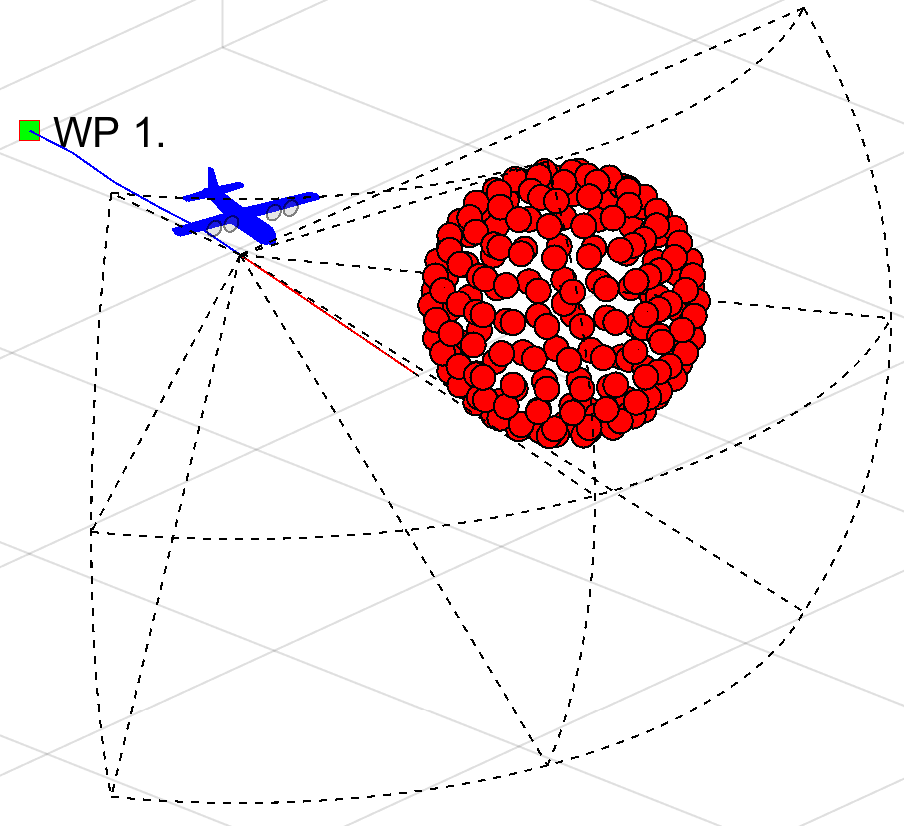
\includegraphics[width=0.75\linewidth]{\FIGDIR/TE038AvoidanceRunExample}        
    \caption{Example: The situation to be evaluated by \emph{Avoidance Run}.}
    \label{fig:exampleSituationAvoidanceRun}
\end{figure}
\newpage
\noindent\emph{Visibility Assessment:} The visibility assessment (fig. \ref{fig:exampleVisibilityEvaluation}) divides the \emph{Avoidance Grid} into two
\begin{enumerate}
    \item \emph{Visible space} (blue filled cells) is space \emph{trough} which \emph{LiDAR} rays roamed freely until they hit an \emph{Obstacle}.
    
    \item \emph{Uncertain space} (black filled cells) is space where no \emph{LiDAR ray} passed nor hit. Therefore its status is uncertain.
\end{enumerate}
 
 \begin{note}
     The \emph{detected obstacle cells} are part of \emph{visible space}, because there is certainty about its containment.
 \end{note}
 
 The \emph{Reach Set} trajectories are colored based on their visibility, blue for \emph{uncertain} trajectories and \emph{green} for visible trajectories.

\begin{figure}[H]
    \centering
    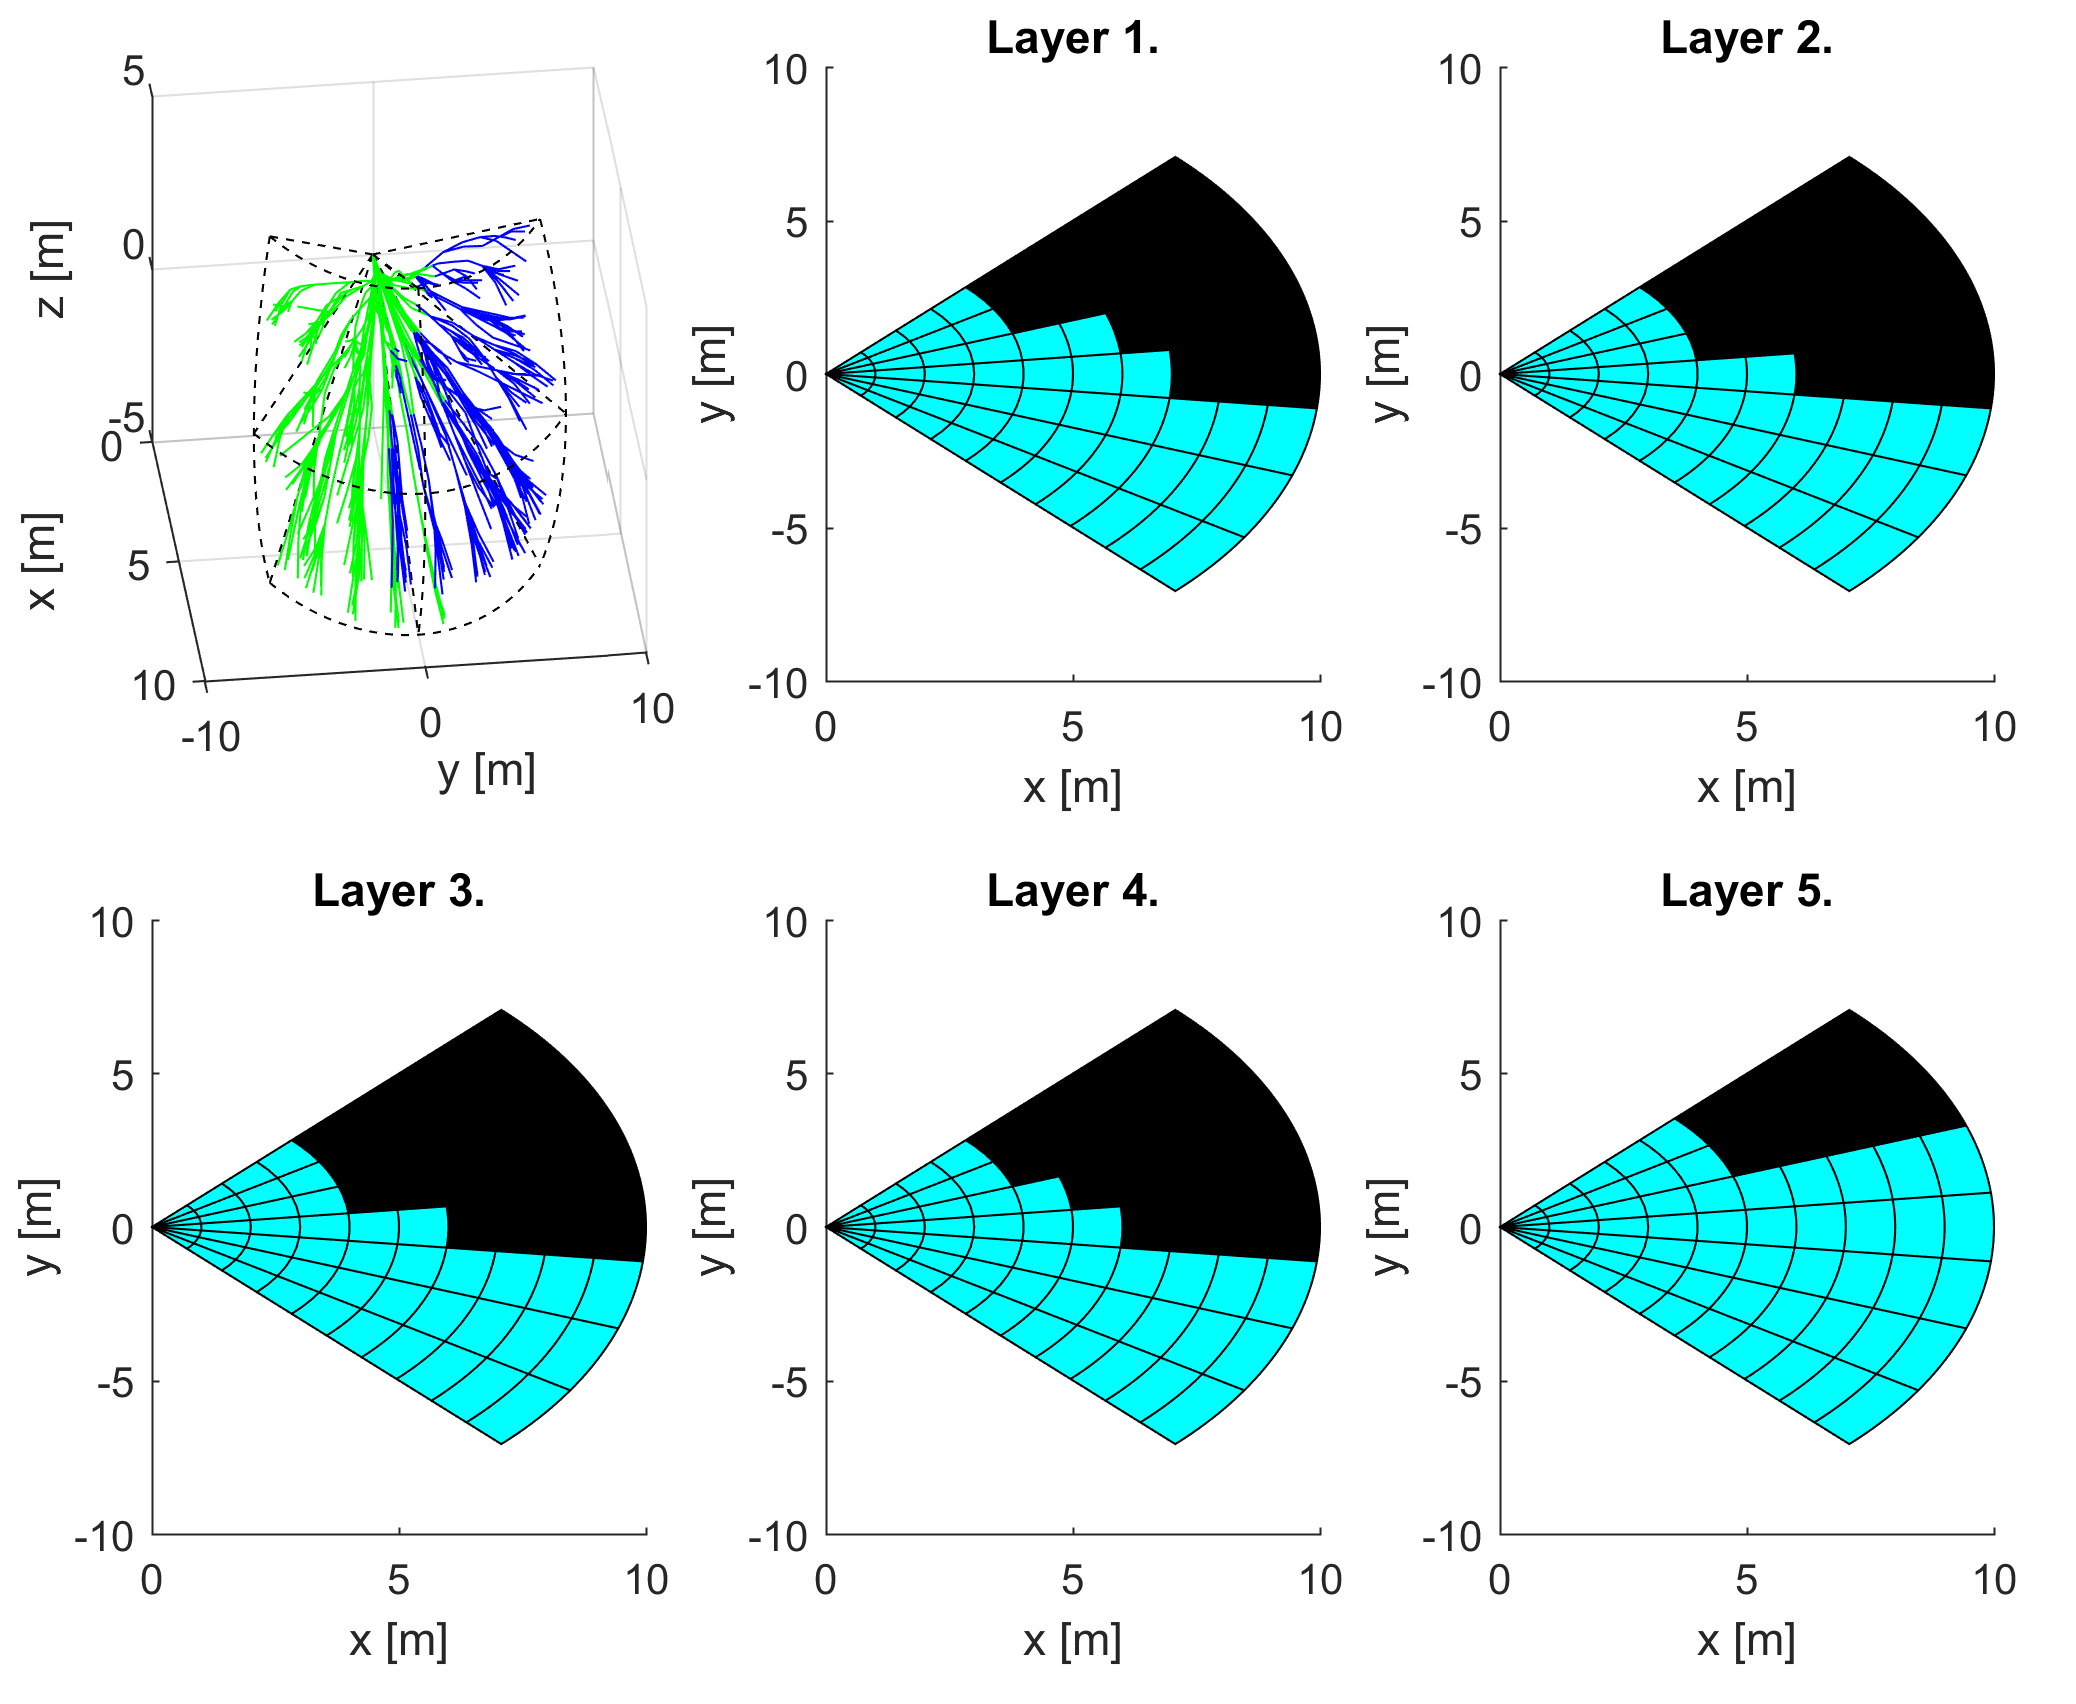
\includegraphics[width=0.95\linewidth]{\FIGDIR/TE040Visibility}        
    \caption{Example: The \emph{Visibility} evaluation by \emph{Avoidance Run}.}
    \label{fig:exampleVisibilityEvaluation}
\end{figure}

\newpage
\noindent\emph{Reachibility Assessment:} For Each trajectory the \emph{Reachibility} is assessed (fig. \ref{fig:exampleReachibilityEvaluation}). The \emph{Obstacle Space} and \emph{Uncertain Space} are rendering \emph{reachibility}, effectively separating \emph{trajectories} into two categories:

\begin{enumerate}
    \item \emph{Unreachable Trajectories} (red lines) - there is at least one trajectory segment leading trough \emph{Obstacle} or \emph{Uncertain} space.
    
    \item \emph{Reachable Trajectories} (green lines) -  all trajectory segments are lying in \emph{Free} space.
\end{enumerate}

Cells in Avoidance grid are divided in similar matter, depending on count of \emph{reachable trajectories} passing trough them:

\begin{enumerate}
    \item \emph{Unreachable Cells} (red fill) - there is no trajectory trough \emph{free space} or the \emph{cell} is not in \emph{free space}.
    
    \item \emph{Reachable cells} (green fill) - there is at least one \emph{feasible trajectory} reaching \emph{free cell}.
\end{enumerate}

\begin{figure}[H]
    \centering
    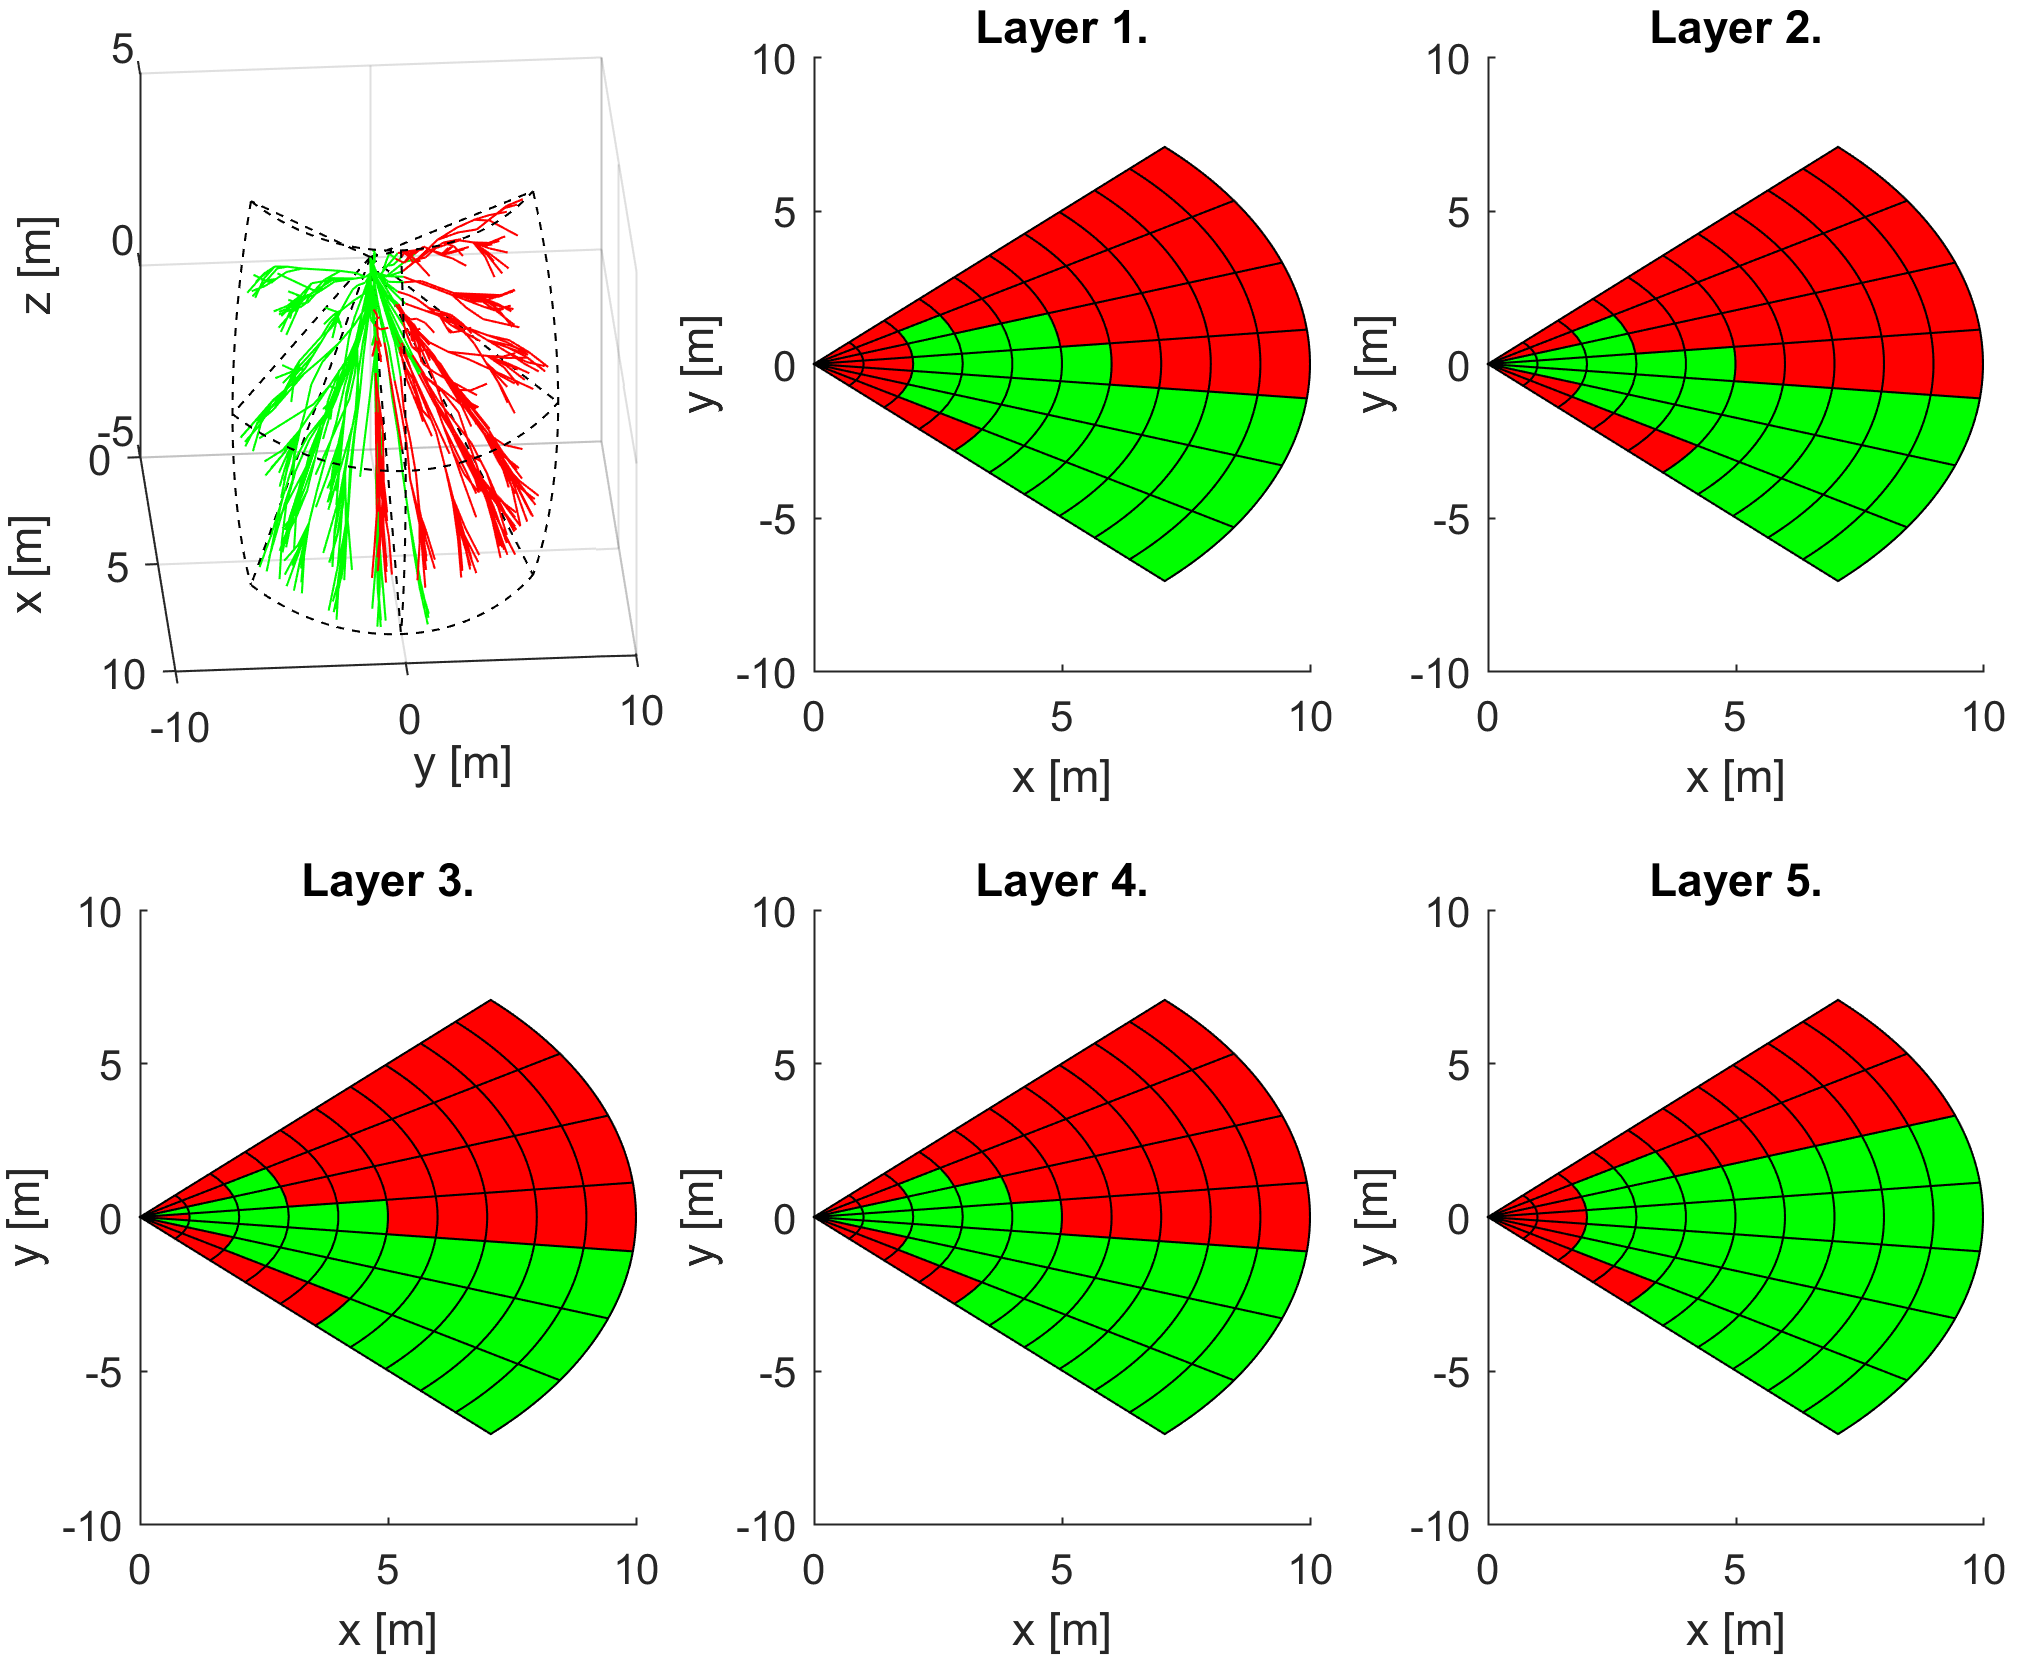
\includegraphics[width=0.95\linewidth]{\FIGDIR/TE041Reachibility}        
    \caption{Example: The \emph{Reachibility} evaluation by \emph{Avoidance Run}.}
    \label{fig:exampleReachibilityEvaluation}
\end{figure}

\begin{note}
    The \emph{best avoidance path} is selected form \emph{reachable outer cells} (green fill in fig. \ref{fig:exampleReachibilityEvaluation}), depending on \emph{goal waypoint} according to (alg. \ref{alg:FindBestPathAvoidanceGrid}).
\end{note}